\documentclass{beamer}
\usepackage{graphicx}
\usepackage{verbatim}
\usepackage{xcolor}
\usepackage{colortbl}

\renewcommand{\figurename}{Gambar}
\renewcommand{\tablename}{Tabel}

\usetheme{metropolis}
\setbeamertemplate{navigation symbols}{}
\usepackage{listings}
\usepackage{xcolor}
\usepackage{ragged2e}

\definecolor{codegreen}{rgb}{0,0.6,0}
\definecolor{codegray}{rgb}{0.5,0.5,0.5}
\definecolor{codepurple}{rgb}{0.58,0,0.82}
\definecolor{backcolour}{rgb}{0.95,0.95,0.92}

\lstset{
    language=Java,
    backgroundcolor=\color{backcolour},   
    commentstyle=\color{codegreen},
    keywordstyle=\color{magenta},
    numberstyle=\tiny\color{codegray},
    stringstyle=\color{codepurple},
    basicstyle=\ttfamily\footnotesize,
    breakatwhitespace=false,         
    breaklines=true,                 
    captionpos=b,                    
    keepspaces=true,                 
    numbers=left,                    
    numbersep=5pt,                  
    showspaces=false,                
    showstringspaces=false,
    showtabs=false,                  
    tabsize=2,
    frame=single,
    columns=flexible
}

\addtobeamertemplate{block begin}{}{\justifying}
\addtobeamertemplate{block begin}{}{\vspace{3px}}

% Info presentasi
\title{Algoritma dan Pemrograman Komputer 1}
\subtitle{Bab 5: Struktur Kontrol I}
\author{Aslam Pandu Tasminto -- 5002241025 \\ M. Ma'ruf Qomaruddin Kafi -- 5002241095}
\date{October 6, 2025}
\institute{Departemen Matematika \\ Fakultas Sains dan Analitika Data \\ Institut Teknologi Sepuluh Nopember}

% Logo untuk title page
\titlegraphic{%
  
\includegraphics[height=0.9cm]{../assets/logoprovikom.jpg}%
  \hspace{0.5em}%
  
\includegraphics[height=0.9cm]{../assets/logomatematika.png}%
  \hspace{0.5em}%
  
\includegraphics[height=1cm]{../assets/logoits.png}%
}

\begin{document}

% Cover
\maketitle

% Daftar Isi
\begin{frame}{Daftar Isi}
  \tableofcontents
\end{frame}

% Section 1: Pengenalan Struktur Kontrol
\section{Pengenalan Struktur Kontrol}
\begin{frame}{Struktur Kontrol dalam Java}
  \begin{block}{Definisi}
    Struktur kontrol adalah pernyataan yang digunakan untuk mengatur alur eksekusi program berdasarkan kondisi tertentu.
  \end{block}
  \begin{block}{Jenis Struktur Kontrol}
    \begin{itemize}
      \item \textbf{Percabangan (Selection)}: if, if-else, if-else if-else, switch
      \item \textbf{Perulangan (Looping)}: for, while, do-while
      \item \textbf{Pengontrol Alur}: break, continue, return
    \end{itemize}
  \end{block}
\end{frame}

\begin{frame}{Pentingnya Struktur Kontrol}
  \begin{figure}[h]
    \centering
    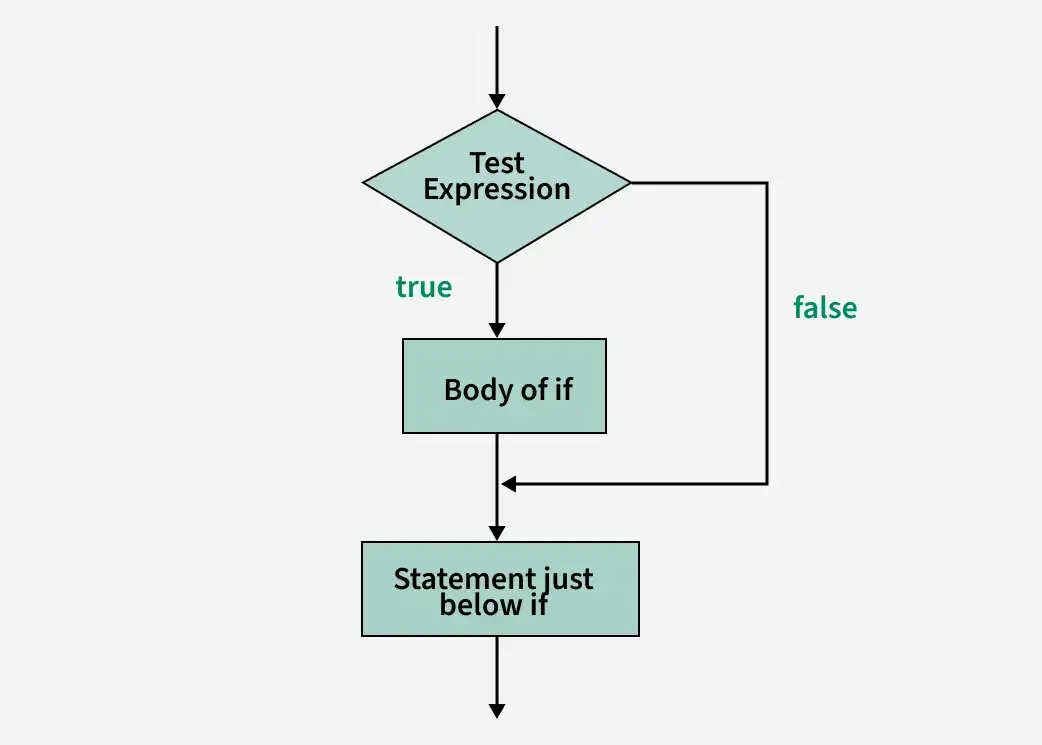
\includegraphics[width=0.7\textwidth]{Struktur Kontrol 1/if-flowchart.png}
    \caption{Diagram alur proses pengambilan keputusan dalam programming}
    \label{fig:flowchart-decision}
  \end{figure}
    \textbf{Sumber: }GeeksforGeeks - Decision Making in Programming
\end{frame}

% Section 2: Pernyataan IF
\section{Pernyataan IF}
\begin{frame}[fragile]{Pernyataan IF Dasar}
  \begin{block}{Sintaks IF Sederhana}
    \begin{lstlisting}
if (kondisi) {
    Pernyataan1 // kode yang dijalankan jika kondisi true
}
    \end{lstlisting}
  \end{block}
  
  \begin{exampleblock}{Contoh Program}
    \begin{lstlisting}
public class CekBilangan {
    public static void main(String[] args) {
        int bilangan = 15;
        if (bilangan > 10) {
            System.out.println("Bilangan lebih besar dari 10");
        }
    }
}\end{lstlisting}
  \end{exampleblock}
\end{frame}

\begin{frame}[fragile]{Contoh Program IF}
\begin{lstlisting}
import java.util.Scanner;

public class IfSederhana {
    public static void main(String[] args) {
        System.out.println("Masukkan sebuah bilangan:");
        Scanner baca = new Scanner(System.in);
        int bil = baca.nextInt();
        
        if (bil >= 10) {
            System.out.println("Ini bukan bilangan kecil");
        }
        System.out.println("Terima kasih");
    }
}
\end{lstlisting}
\end{frame}

\begin{frame}[fragile]{Output Program IF}
\begin{block}{Contoh Eksekusi Program}
\colorbox{gray!20}{
    \parbox{0.9\textwidth}{
        \texttt{Masukkan sebuah bilangan: \textbf{15}\\
        Ini bukan bilangan kecil\\
        Terima kasih}
    }
}
\end{block}

\begin{block}{Penjelasan}
\begin{itemize}
\item User memasukkan bilangan: \textbf{15}
\item Karena 15 $\geq$ 10 bernilai \textbf{true}
\item Program mengeksekusi \texttt{"Ini bukan bilangan kecil"}
\item Statement \texttt{"Terima kasih"} selalu dieksekusi (di luar blok if)
\end{itemize}
\end{block}
\end{frame}

% Section 3: IF-ELSE
\section{IF-ELSE}
\begin{frame}[fragile]{Pernyataan IF-ELSE}
  \begin{block}{Sintaks IF-ELSE}
    \begin{lstlisting}
if (kondisi) {
    // kode jika kondisi true
} else {
    // kode jika kondisi false
}
    \end{lstlisting}
  \end{block}
\end{frame}

\begin{frame}{Pernyataan IF-ELSE}
    \begin{figure}[h]
    \centering
    % includegraphics[width=0.75\linewidth]{Struktur Kontrol 1/if-else-flowchart.png}
    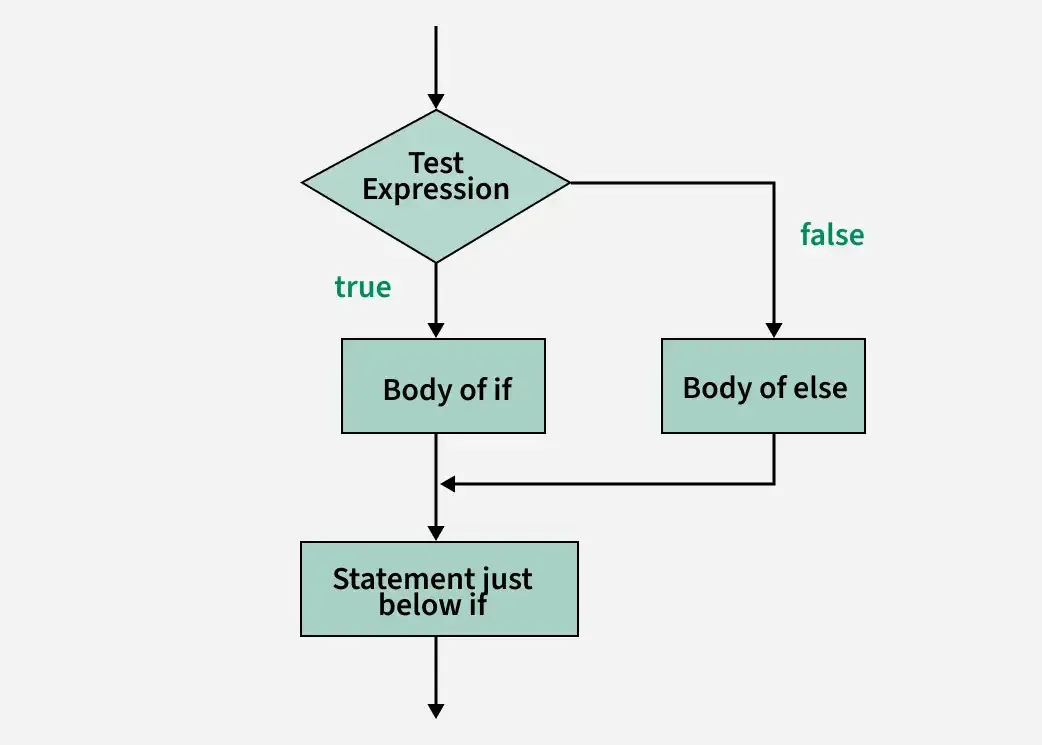
\includegraphics[width=0.5\linewidth]{Struktur Kontrol 1/if-else-flowchart.png}
    \caption{Alur eksekusi pernyataan if-else}
    \label{fig:if-else-flow}
  \end{figure}
  \textbf{Sumber: }GeeksforGeeks - Decision Making in Programming
\end{frame}

\begin{frame}[fragile]{Contoh Program IF-ELSE}
\begin{lstlisting}
import java.util.Scanner;

public class CekNilaiAlpro {
    public static void main(String[] args) {
        System.out.println("Masukkan nilai Algoritma Pemrograman:");
        Scanner baca = new Scanner(System.in);
        double nilai = baca.nextDouble();
        
        if (nilai >= 76) {
            System.out.println("keren banget maniez :)");
        } else {
            System.out.println("belajar lagi yaa maniez :(");
        }
    }
}
\end{lstlisting}
\end{frame}

\begin{frame}{Output Program IF-ELSE}
\begin{block}{Contoh Eksekusi Program}
\colorbox{gray!20}{
    \parbox{0.9\textwidth}{
        \texttt{Masukkan nilai Algoritma Pemrograman: \textbf{85}\\
        keren banget maniez :)}
    }
}
\end{block}

\begin{block}{Contoh Lain}
\colorbox{gray!20}{
    \parbox{0.9\textwidth}{
        \texttt{Masukkan nilai Algoritma Pemrograman: \textbf{65}\\
        belajar lagi yaa maniez :(}
    }
}
\end{block}

\begin{block}{Penjelasan}
\begin{itemize}
\item Jika nilai $\geq$ 76: menampilkan pesan positif dengan emoticon senang
\item Jika nilai $<$ 76: menampilkan pesan motivasi dengan emoticon sedih
\item Hanya satu blok yang dieksekusi (if ATAU else)
\end{itemize}
\end{block}
\end{frame}

% Section 4: IF-ELSE IF-ELSE
\section{IF-ELSE IF-ELSE}
\begin{frame}[fragile]{Pernyataan IF-ELSE IF-ELSE}
  \begin{block}{Sintaks Multi Kondisi}
    \begin{lstlisting}
if (kondisi1) {
    // kode jika kondisi1 true
} else if (kondisi2) {
    // kode jika kondisi2 true
} else if (kondisi3) {
    // kode jika kondisi3 true
} else {
    // kode jika semua kondisi false
}
    \end{lstlisting}
  \end{block}
\end{frame}

\section{IF-ELSE IF-ELSE}
\begin{frame}[fragile]{Pernyataan IF-ELSE IF-ELSE}
  \begin{block}{Sintaks Multi Kondisi}
    \begin{lstlisting}
if (kondisi1) {
    // kode jika kondisi1 true
} else if (kondisi2) {
    // kode jika kondisi2 true
} else if (kondisi3) {
    // kode jika kondisi3 true
} else {
    // kode jika semua kondisi false
}
    \end{lstlisting}
  \end{block}
\end{frame}

\begin{frame}{Flowchart IF-ELSE IF-ELSE}
  \begin{figure}[h]
    \centering
    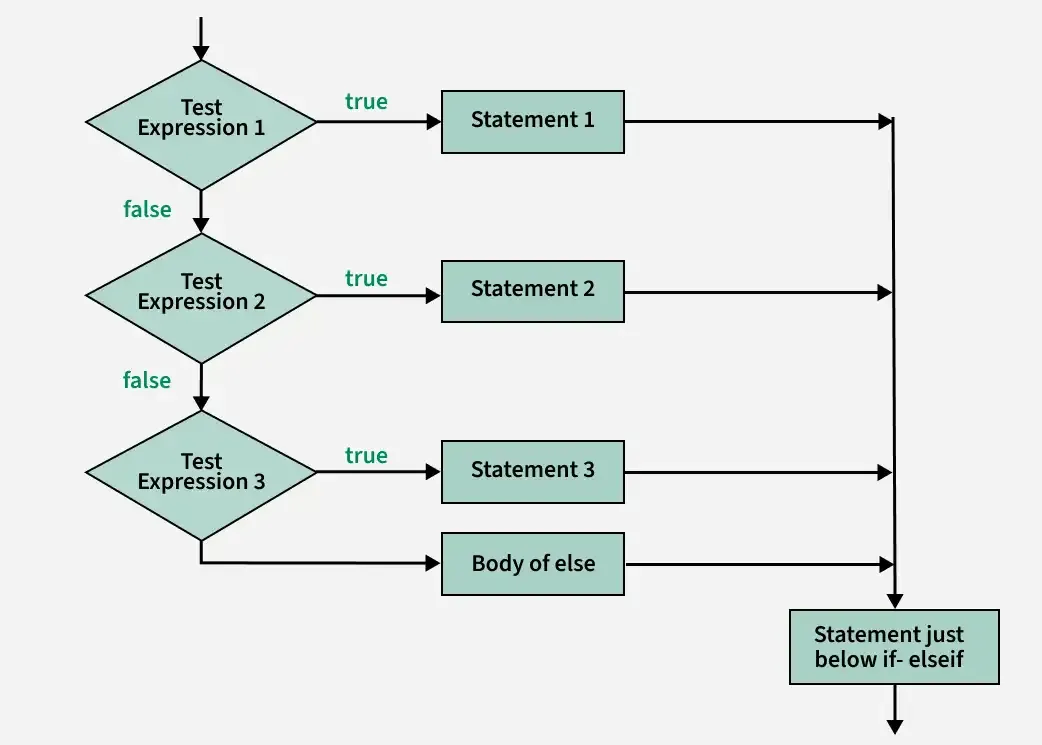
\includegraphics[width=0.7\linewidth]{Struktur Kontrol 1/if-elseif-else.png}
    \caption{Alur eksekusi pernyataan IF-ELSE IF-ELSE}
    \label{fig:if-else-if-flow}
  \end{figure}
  \textbf{Sumber:} GeeksforGeeks - Decision Making in Programming
\end{frame}

\begin{frame}{Karakteristik IF-ELSE IF-ELSE}
\begin{block}{Karakteristik IF-ELSE IF-ELSE}
    \begin{itemize}
      \item Dievaluasi secara berurutan dari atas ke bawah
      \item Hanya satu blok yang akan dieksekusi
      \item Evaluasi berhenti ketika menemukan kondisi yang true
      \item Blok \texttt{else} bersifat opsional
    \end{itemize}
  \end{block}
\end{frame}
\begin{frame}[fragile]{Contoh Program IF-ELSE IF-ELSE}
\begin{lstlisting}
import java.util.Scanner;

public class KonversiNilai {
    public static void main(String[] args) {
        System.out.println("Masukkan nilai angka anda:");
        Scanner baca = new Scanner(System.in);
        int nilai = baca.nextInt();
        
        if (nilai >= 86 && nilai <= 100) {
            System.out.println("Nilai Huruf Anda A / Istimewa");
        } else if (nilai >= 76 && nilai <= 85) {
            System.out.println("Nilai Huruf Anda AB / Baik Sekali");
        } else if (nilai >= 66 && nilai <= 75) {
            System.out.println("Nilai Huruf Anda B / Baik");
        }
\end{lstlisting}
\end{frame}

\begin{frame}[fragile]{Contoh Program IF-ELSE IF-ELSE}
\begin{lstlisting}
        else if (nilai >= 61 && nilai <= 65) {
            System.out.println("Nilai Huruf Anda BC / Cukup Baik");
        } else if (nilai >= 56 && nilai <= 60) {
            System.out.println("Nilai Huruf Anda C / Cukup");
        } else if (nilai >= 41 && nilai <= 55) {
            System.out.println("Nilai Huruf Anda D / Kurang");
        } else if (nilai >= 0 && nilai <= 40) {
            System.out.println("Nilai Huruf Anda E / Kurang Sekali");
        } else {
            System.out.println("Nilai tidak valid!");
        }
    }
}
\end{lstlisting}
\end{frame}

\begin{frame}{Tabel Rentang Nilai Berdasarkan Peraturan Akademik 2018}
  \begin{table}
    \footnotesize
    \begin{tabular}{p{0.25\textwidth}|p{0.25\textwidth}|p{0.4\textwidth}}
    \textbf{Rentang Nilai} & \textbf{Nilai Huruf} & \textbf{Keterangan} \\
    \hline
    \rowcolor{lightgray}
    86 - 100 & A & Istimewa \\
    \rowcolor{white}
    76 - 85 & AB & Baik Sekali \\
    \rowcolor{lightgray}
    66 - 75 & B & Baik \\
    \rowcolor{white}
    61 - 65 & BC & Cukup Baik \\
    \rowcolor{lightgray}
    56 - 60 & C & Cukup \\
    \rowcolor{white}
    41 - 55 & D & Kurang \\
    \rowcolor{lightgray}
    0 - 40 & E & Kurang Sekali \\
    \end{tabular}
    \caption{Tabel konversi nilai berdasarkan Peraturan Akademik ITS}
  \end{table}
\end{frame}

\begin{frame}{Output Program IF-ELSE IF-ELSE}
\begin{block}{Contoh Eksekusi Program}
\colorbox{gray!20}{
    \parbox{0.9\textwidth}{
        \texttt{Masukkan nilai angka anda: \textbf{92}\\
        Nilai Huruf Anda A / Istimewa}
    }
}
\end{block}

\begin{block}{Contoh Lain}
\colorbox{gray!20}{
    \parbox{0.9\textwidth}{
        \texttt{Masukkan nilai angka anda: \textbf{78}\\
        Nilai Huruf Anda AB / Baik Sekali\\
        \\
        Masukkan nilai angka anda: \textbf{63}\\
        Nilai Huruf Anda BC / Cukup Baik\\
        \\
        Masukkan nilai angka anda: \textbf{35}\\
        Nilai Huruf Anda E / Kurang Sekali}
    }
}
\end{block}
\end{frame}

% Section 5: Nested IF
\section{Nested IF}
\begin{frame}[fragile]{Nested IF (IF Bersarang)}
  \begin{block}{Konsep Nested IF}
    \begin{itemize}
      \item IF di dalam IF
      \item Digunakan untuk kondisi yang kompleks
      \item Setiap kondisi harus dipenuhi secara berurutan
    \end{itemize}
  \end{block}

  \begin{exampleblock}{Sintaks Nested IF}
    \begin{lstlisting}
if (kondisi1) {
    if (kondisi2) {
        // kode jika kedua kondisi true
    }
}
    \end{lstlisting}
  \end{exampleblock}
\end{frame}

\begin{frame}{Flowchart Nested IF}
  \begin{figure}
      \centering
      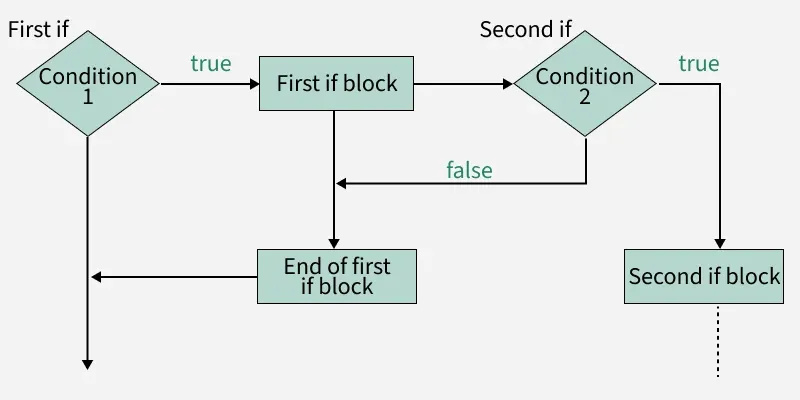
\includegraphics[width=0.75\linewidth]{Struktur Kontrol 1/nested-if-flowchart.png}
      \caption{Alur eksekusi Nested IF (IF Bersarang)}
      \label{fig:placeholder}
  \end{figure}
  \textbf{Sumber: }GeeksforGeeks - Decision Making in Programming
\end{frame}

\begin{frame}{Karakteristid Nested IF}
  \begin{block}{Karakteristik Nested IF}
    \begin{itemize}
      \item Kondisi dievaluasi secara bertingkat
      \item Kondisi IF ke-2 hanya dieksekusi jika kondisi IF ke-1 bernilai true
      \item Cocok untuk validasi bertingkat
    \end{itemize}
  \end{block}
\end{frame}
\begin{frame}[fragile]{Contoh Program Nested IF}
\begin{lstlisting}
import java.util.Scanner;

public class MenuProgram {
    public static void main(String[] args) {
        Scanner baca = new Scanner(System.in);
        
        System.out.println("Pilih program:");
        System.out.println("1. Cek Bilangan");
        System.out.println("2. Cek Nilai");
        System.out.println("3. Keluar");
        System.out.print("Masukkan pilihan (1-3): ");
        
        int pilihan = baca.nextInt();
        
        if (pilihan == 1) {
            System.out.print("Masukkan bilangan: ");
            int bil = baca.nextInt();
\end{lstlisting}
\end{frame}

\begin{frame}[fragile]{Contoh Program Nested IF}
\begin{lstlisting}
            if (bil >= 10) {
                System.out.println("Bilangan BESAR");
            } else {
                System.out.println("Bilangan KECIL");
            }
            
        } else if (pilihan == 2) {
            System.out.print("Masukkan nilai: ");
            double nilai = baca.nextDouble();
            
            if (nilai >= 76) {
                System.out.println("LULUS - Keren!");
            } else {
                System.out.println("REMIDIAL - Semangat!");
            }
\end{lstlisting}
\end{frame}

\begin{frame}[fragile]{Contoh Program Nested IF}
\begin{lstlisting} 
        } else if (pilihan == 3) {
            System.out.println("Terima kasih!");
            
        } else {
            System.out.println("Pilihan tidak valid!");
        }
    }
}
\end{lstlisting}
\end{frame}
\begin{frame}{Output Program Nested IF}
\begin{block}{Contoh 1: Cek Bilangan}
\colorbox{gray!20}{
    \parbox{0.9\textwidth}{
        \footnotesize\texttt{Pilih program:\\
        1. Cek Bilangan\\
        2. Cek Nilai\\
        3. Keluar\\
        Masukkan pilihan (1-3): \textbf{1}\\
        Masukkan bilangan: \textbf{15}\\
        Bilangan BESAR}
    }
}
\end{block}

\begin{block}{Contoh 2: Cek Nilai}
\colorbox{gray!20}{
    \parbox{0.9\textwidth}{
        \footnotesize\texttt{Pilih program:\\
        1. Cek Bilangan\\
        2. Cek Nilai\\
        3. Keluar\\
        Masukkan pilihan (1-3): \textbf{2}\\
        Masukkan nilai: \textbf{65}\\
        REMIDIAL - Semangat!}
    }
}
\end{block}
\end{frame}

\begin{frame}{Output Program Nested IF}
\begin{block}{Contoh 3: Keluar Program}
\colorbox{gray!20}{
    \parbox{0.9\textwidth}{
        \footnotesize\texttt{Pilih program:\\
        1. Cek Bilangan\\
        2. Cek Nilai\\
        3. Keluar\\
        Masukkan pilihan (1-3): \textbf{3}\\
        Terima kasih!}
    }
}
\end{block}

\begin{block}{Contoh 4: Pilihan Invalid}
\colorbox{gray!20}{
    \parbox{0.9\textwidth}{
        \footnotesize\texttt{Pilih program:\\
        1. Cek Bilangan\\
        2. Cek Nilai\\
        3. Keluar\\
        Masukkan pilihan (1-3): \textbf{5}\\
        Pilihan tidak valid!}
    }
}
\end{block}
\end{frame}

\begin{frame}{Penjelasan Output Program Nested IF}
\begin{block}{Penjelasan}
\begin{itemize}
\item \textbf{IF 1}: Validasi pilihan menu (1, 2, 3)
\item \textbf{IF 2}: Jika pilihan valid, eksekusi secara spesifik
\item Setiap menu memiliki nested if untuk logika internal
\end{itemize}
\end{block}
\end{frame}

% Section 6: IF Bersebelahan
\section{Sequential IF}
\begin{frame}[fragile]{Sequential IF (IF Bersebelahan)}
  \begin{block}{Konsep IF Bersebelahan}
    \begin{itemize}
      \item Beberapa pernyataan IF yang berurutan
      \item Setiap IF dievaluasi secara independen
      \item Bisa beberapa kondisi yang true sekaligus
    \end{itemize}
  \end{block}
\end{frame}

\begin{frame}[fragile]{Contoh Program IF Bersebelahan}
\begin{lstlisting}
import java.util.Scanner;

public class ValidasiInput {
    public static void main(String[] args) {
        System.out.println("Masukkan nilai (0-100):");
        Scanner baca = new Scanner(System.in);
        int bilangan = baca.nextInt();
        
        // IF bersebelahan - semua dievaluasi
        if (bilangan > 100) {
            System.out.println("Nilai terlalu besar");
        }
\end{lstlisting}
\end{frame}

\begin{frame}[fragile]{Contoh Program IF Bersebelahan}
\begin{lstlisting}
        if (bilangan < 0) {
            System.out.println("Nilai terlalu kecil");
        }
        if (bilangan >= 0 && bilangan <= 100) {
            System.out.println("Nilai sesuai");
        }
    }
}
\end{lstlisting}
\end{frame}

\begin{frame}{Perbandingan IF Bertingkat vs IF Bersebelahan}
  \begin{table}
    \footnotesize
    \begin{tabular}{p{0.45\textwidth}|p{0.45\textwidth}}
    \textbf{IF Bertingkat} & \textbf{IF Bersebelahan} \\
    \hline
    \rowcolor{lightgray}
    Hanya satu blok yang dieksekusi & Banyak blok bisa dieksekusi \\
    \rowcolor{white}
    Evaluasi berhenti saat kondisi true & Semua kondisi dievaluasi \\
    \rowcolor{lightgray}
    Efisien untuk pilihan bergantian & Fleksibel untuk pengecekan terpisah \\
    \rowcolor{white}
    Cocok untuk klasifikasi & Cocok untuk validasi \\
    \end{tabular}
    \caption{Perbandingan IF bertingkat dan IF bersebelahan}
  \end{table}
\end{frame}

% Section 7: Operator Logika dalam IF
\section{Operator Logika dalam IF}
\begin{frame}[fragile]{Operator Logika untuk Kondisi Kompleks}
  \begin{block}{Operator Logika yang Sering Digunakan}
    \begin{lstlisting}
// AND (&&) - kedua kondisi harus true
if (nilai >= 60 && nilai <= 100) {
    System.out.println("Lulus");
}

// OR (||) - salah satu kondisi true
if (hari == "Sabtu" || hari == "Minggu") {
    System.out.println("Weekend");
}

// NOT (!) - negasi
if (!isTamat) {
    System.out.println("Belum tamat");
}
    \end{lstlisting}
  \end{block}
\end{frame}

\begin{frame}{Tabel Operator Logika}
  \begin{table}
    \footnotesize
    \begin{tabular}{p{0.15\textwidth}|p{0.2\textwidth}|p{0.55\textwidth}}
    \textbf{Operator} & \textbf{Contoh} & \textbf{Deskripsi} \\
    \hline
    \rowcolor{lightgray}
    \&\& & a \&\& b & True jika a DAN b true \\
    \rowcolor{white}
    \textbar\textbar & a \textbar\textbar b & True jika a ATAU b true \\
    \rowcolor{lightgray}
    ! & !a & True jika a false, dan sebaliknya \\
    \rowcolor{white}
    == & a == b & True jika a sama dengan b \\
    \rowcolor{lightgray}
    != & a != b & True jika a tidak sama dengan b \\
    \rowcolor{white}
    $>$, $<$ & a $>$ b & Membandingkan nilai lebih besar/lebih kecil \\
    \rowcolor{lightgray}
    $>=$, $<=$ & a $>=$ b & Membandingkan nilai lebih besar/kecil sama dengan \\
    \end{tabular}
    \caption{Operator logika dan perbandingan dalam Java}
  \end{table}
\end{frame}
% Section 8: Latihan
\section{Latihan}
\begin{frame}{Latihan 1: Penentu Kelulusan}
  \begin{block}{Soal 1: Penentu Kelulusan}
    Buat program yang meminta input:
    \begin{itemize}
      \item Nilai ujian (0-100)
      \item Kehadiran (persentase 0-100\%)
    \end{itemize}
    Kelulusan ditentukan oleh:
    \begin{itemize}
      \item Lulus jika: nilai $\geq$ 60 DAN kehadiran $\geq$ 75\%
      \item Remedial jika: nilai $\geq$ 40 DAN kehadiran $\geq$ 75\%
      \item Tidak lulus untuk kondisi lainnya
    \end{itemize}
  \end{block}
\end{frame}

\begin{frame}{Latihan 2: Kategori Usia}
  \begin{block}{Soal 2: Kategori Usia}
    Buat program yang mengkategorikan usia:
    \begin{itemize}
      \item Anak-anak: 0-12 tahun
      \item Remaja: 13-17 tahun  
      \item Dewasa muda: 18-25 tahun
      \item Dewasa: 26-45 tahun
      \item Lansia: $>$45 tahun
    \end{itemize}
    Gunakan struktur if-else if-else!
  \end{block}
\end{frame}

\begin{frame}{Latihan 3: Kalkulator Sederhana}
  \begin{block}{Soal 3: Kalkulator Sederhana}
    Buat program kalkulator yang:
    \begin{itemize}
      \item Meminta input 2 bilangan
      \item Meminta operator (+, -, *, /, \%)
      \item Menggunakan nested if untuk validasi:
        \begin{itemize}
          \item Jika operator '/', cek pembagi tidak boleh 0
          \item Jika operator tidak valid, tampilkan pesan error
        \end{itemize}
      \item Tampilkan hasil operasi
    \end{itemize}
  \end{block}
\end{frame}

% Section 9: Kesimpulan
\section{Kesimpulan}
\begin{frame}{Kesimpulan}
  \begin{alertblock}{Inti Bab 5: Struktur Kontrol I}
    \begin{itemize}
      \item \textbf{IF} digunakan untuk eksekusi kode berdasarkan kondisi boolean
      \item \textbf{IF-ELSE} memberikan alternatif ketika kondisi false
      \item \textbf{IF-ELSE IF-ELSE} menangani multiple kondisi secara berurutan
      \item \textbf{Nested IF} untuk kondisi yang kompleks dan bertingkat
      \item \textbf{Sequential IF} untuk kondisi yang independen dan perlu semua dievaluasi
      \item Pemilihan struktur kontrol tergantung pada logika program yang dibutuhkan
    \end{itemize}
  \end{alertblock}
\end{frame}

% Section 10: Referensi
\section{Referensi}
\begin{frame}{Referensi}
  \begin{block}{Referensi:}
    \begin{itemize}
      \item \textbf{Modul Praktikum Algoritma dan Pemrograman}\\
            Departemen Matematika FSAD ITS
      \item \textbf{Oracle Java Tutorials - Control Flow Statements}\\
            \url{https://docs.oracle.com/javase/tutorial/java/nutsandbolts/flow.html}
      \item \textbf{GeeksforGeeks - Decision Making in Java}\\
            \url{https://www.geeksforgeeks.org/decision-making-javaif-else-switch-break-continue-jump/}
    \end{itemize}
  \end{block}
\end{frame}

% Penutup
\begin{frame}[standout]
  \Huge \textbf{Terima Kasih} \\[1.5em]
  \Large Pertanyaan dan Diskusi
\end{frame}

\end{document}